\documentclass[11pt]{article}
\usepackage{microtype}
\usepackage{graphicx}
\usepackage{wrapfig}
\usepackage{url}
\usepackage{wrapfig}
\usepackage{color}
\usepackage{marvosym}
\usepackage{enumerate}
\usepackage{subfigure}
\usepackage{tikz}
\usepackage[fleqn]{amsmath}
\DeclareMathOperator*{\argmax}{arg\,max}
\DeclareMathOperator*{\argmin}{arg\,min}
\usepackage{amssymb}
\usepackage{hyperref}
\usepackage[many]{tcolorbox}
\usepackage{lipsum}
\usepackage{float}
\usepackage{trimclip}
\usepackage{listings}
\usepackage{environ}% http://ctan.org/pkg/environ
\usepackage{wasysym}
\usepackage{array}
\usepackage{cancel}

\newcommand{\Angie}[1]{\textcolor{blue}{Angie - #1}}
\newcommand{\Xuan}[1]{\textcolor{green}{Xuan - #1}}


\oddsidemargin 0mm
\evensidemargin 5mm
\topmargin -20mm
\textheight 240mm
\textwidth 160mm

\newcommand{\vwi}{{\bf w}_i}
\newcommand{\vw}{{\bf w}}
\newcommand{\vx}{{\bf x}}
\newcommand{\vy}{{\bf y}}
\newcommand{\vxi}{{\bf x}_i}
\newcommand{\yi}{y_i}
\newcommand{\vxj}{{\bf x}_j}
\newcommand{\vxn}{{\bf x}_n}
\newcommand{\yj}{y_j}
\newcommand{\ai}{\alpha_i}
\newcommand{\aj}{\alpha_j}
\newcommand{\X}{{\bf X}}
\newcommand{\Y}{{\bf Y}}
\newcommand{\vz}{{\bf z}}
\newcommand{\msigma}{{\bf \Sigma}}
\newcommand{\vmu}{{\bf \mu}}
\newcommand{\vmuk}{{\bf \mu}_k}
\newcommand{\msigmak}{{\bf \Sigma}_k}
\newcommand{\vmuj}{{\bf \mu}_j}
\newcommand{\msigmaj}{{\bf \Sigma}_j}
\newcommand{\pij}{\pi_j}
\newcommand{\pik}{\pi_k}
\newcommand{\D}{\mathcal{D}}
\newcommand{\el}{\mathcal{L}}
\newcommand{\N}{\mathcal{N}}
\newcommand{\vxij}{{\bf x}_{ij}}
\newcommand{\vt}{{\bf t}}
\newcommand{\yh}{\hat{y}}
\newcommand{\code}[1]{{\footnotesize \tt #1}}
\newcommand{\alphai}{\alpha_i}
\newcommand{\defeq}{\overset{\text{def}}{=}}
\renewcommand{\vec}[1]{\mathbf{#1}}



\bgroup
\def\arraystretch{1.5}
\newcolumntype{x}[1]{>{\centering\arraybackslash\hspace{0pt}}p{#1}}
\newcolumntype{z}[1]{>{\centering\arraybackslash}m{#1}}

%Arguments are 1 - height, 2 - box title
\newtcolorbox{textanswerbox}[2]{%
 width=\textwidth,colback=white,colframe=blue!30!black,floatplacement=H,height=#1,title=#2,clip lower=true,before upper={\parindent0em}}

 \newtcolorbox{eqanswerbox}[1]{%
 width=#1,colback=white,colframe=black,floatplacement=H,height=3em,sharp corners=all,clip lower=true,before upper={\parindent0em}}

 %Arguments are 1 - height, 2 - box title
 \NewEnviron{answertext}[2]{
        \noindent
        \marginbox*{0pt 10pt}{
        \clipbox{0pt 0pt 0pt 0pt}{
        \begin{textanswerbox}{#1}{#2}
        \BODY
        \end{textanswerbox}
        }
        }
}

%Arguments are 1 - height, 2 - box title, 3 - column definition
 \NewEnviron{answertable}[3]{
        \noindent
        \marginbox*{0pt 10pt}{
        \clipbox{0pt 0pt 0pt 0pt}{
        \begin{textanswerbox}{#1}{#2}
                \vspace{-0.5cm}
                        \begin{table}[H]
                        \centering
                        \begin{tabular}{#3}
                                \BODY
                        \end{tabular}
                        \end{table}
        \end{textanswerbox}
        }
        }
}

 %Arguments are 1 - height, 2 - box title, 3 - title, 4- equation label, 5 - equation box width
 \NewEnviron{answerequation}[5]{
        \noindent
        \marginbox*{0pt 10pt}{
        \clipbox{0pt 0pt 0pt 0pt}{
        \begin{textanswerbox}{#1}{#2}
                \vspace{-0.5cm}
                        \begin{table}[H]
                        \centering
                \renewcommand{\arraystretch}{0.5}% Tighter

                        \begin{tabular}{#3}
                                #4 =	&
                        \clipbox{0pt 0pt 0pt 0pt}{

                        \begin{eqanswerbox}{#5}
                                $\BODY$
                        \end{eqanswerbox}
                        } \\
                        \end{tabular}
                        \end{table}

        \end{textanswerbox}
        }
        }
}

 %Arguments are 1 - height, 2 - box title
 \NewEnviron{answerderivation}[2]{
        \noindent
        \marginbox*{0pt 10pt}{
        \clipbox{0pt 0pt 0pt 0pt}{
        \begin{textanswerbox}{#1}{#2}
        \BODY
        \end{textanswerbox}
        }
        }
}

\newcommand{\Checked}{{\LARGE \XBox}}%
\newcommand{\Unchecked}{{\LARGE \Square}}%
\newcommand{\TextRequired}{{\textbf{Place Answer Here}}}%
\newcommand{\EquationRequired}{\textbf{Type Equation Here}}%


\newcommand{\answertextheight}{5cm}
\newcommand{\answertableheight}{4cm}
\newcommand{\answerequationheight}{2.5cm}
\newcommand{\answerderivationheight}{14cm}

\newcounter{QuestionCounter}
\newcounter{SubQuestionCounter}[QuestionCounter]
\setcounter{SubQuestionCounter}{1}

\newcommand{\subquestiontitle}{Question \theQuestionCounter.\theSubQuestionCounter~}
\newcommand{\newquestion}{\stepcounter{QuestionCounter}\setcounter{SubQuestionCounter}{1}\newpage}
\newcommand{\newsubquestion}{\stepcounter{SubQuestionCounter}}


\lstset{language=[LaTeX]TeX,basicstyle=\ttfamily\bf}

\pagestyle{myheadings}
\markboth{Homework 4}{Fall 2022 CS 475/675 Machine Learning: Homework 4}

\title{CS 475/675 Machine Learning: Homework 4\\
Analytical Questions\\
\Large{30 Points Total \hspace{1cm} Version 2.0}
\author{PARTNER1\_NAME, PARTER2\_NAME, $\ldots$ \\
PARTNER1\_JHED, PARTNER2\_JHED, $\ldots$}}
\date{}

\begin{document}
\maketitle
\thispagestyle{headings}


\section*{Instructions }
We have provided this \LaTeX{} document for completing the analytical portion of the assignment. We give you one or more boxes to answer each question.  The question to answer for each box will be noted in the title of the box.\\

{\bf Other than your name, do not type anything outside the boxes. Leave the rest of the document unchanged.}\\


\textbf{Do not change any formatting in this document, or we may be unable to
  grade your work. This includes, but is not limited to, the height of
  textboxes, font sizes, and the spacing of text and tables.  Additionally, do
  not add text outside of the answer boxes. Entering your answers are the only
  changes allowed.}\\


\textbf{We strongly recommend you review your answers in the generated PDF to
  ensure they appear correct. We will grade what appears in the answer boxes in
  the submitted PDF, NOT the original latex file.}

\pagebreak

\newquestion
\section*{\arabic{QuestionCounter}) 
LSTM (9 points)} 
In this question, we will compare three parameterizations of a LSTM using different gating mechanisms: 1) the vanilla LSTM, 2) peephole LSTM and 3) tanh-LSTM.

\noindent \textbf{Vanilla LSTM} We begin by defining a vanilla LSTM as follows. Given the input vector at time $t$ as $\mathbf{x}_t$, the variables and gates are defined as follows:
\begin{align}
    \label{eq1} &\mathbf{g}_t = \tanh(\mathbf{W}_{gx}\mathbf{x}_t+\mathbf{W}_{gh}\mathbf{h}_{t-1} + \mathbf{b}_g)\\ 
    \label{eq2} &\mathbf{i}_t = \sigma(\mathbf{W}_{ix}\mathbf{x}_t+\mathbf{W}_{ih}\mathbf{h}_{t-1}+\mathbf{b}_i) \\
    \label{eq3} &\mathbf{f}_t = \sigma(\mathbf{W}_{fx}\mathbf{x}_t + \mathbf{W}_{fh}\mathbf{h}_{t-1} + \mathbf{b}_f)\\
    \label{eq4} &\mathbf{c}_t = \mathbf{f}_t \odot \mathbf{c}_{t-1} + \mathbf{i}_t \odot \mathbf{g}_t \\
    \label{eq5} &\mathbf{o}_t = \sigma(\mathbf{W}_{ox}\mathbf{x}_t + \mathbf{W}_{oh}\mathbf{h}_{t-1}+\mathbf{b}_o)\\
    \label{eq6} &\mathbf{h}_t = \mathbf{o}_t \odot \tanh(\mathbf{c}_t).
\end{align}
Here, $\mathbf{g}$ is the block input, $\mathbf{i}$, $\mathbf{f}$, and $\mathbf{o}$ are respectively the input, forget, and output gates, $\mathbf{c}$ represents the memory cell value, and $\mathbf{h}$ is the block output. $\mathbf{W}_{**}$ are weights. $\mathbf{b}_{*}$ are biases. $\sigma$ is the sigmoid function. $\odot$ denotes the element-wise Hadamard product. \\\\
\textbf{Peephole LSTM} enriches the vanilla LSTM by enabling the memory cell $\mathbf{c}$ to influence the value of the gates through a set of recurrent weights $\mathbf{W}_{*c}$. For the peephole LSTM, Equation \eqref{eq1} \eqref{eq4} \eqref{eq6} remain unchanged, while the gates \eqref{eq2} \eqref{eq3} \eqref{eq5} become:
\begin{align}
    \label{eq7} &\mathbf{i}_t = \sigma(\mathbf{W}_{ix}\mathbf{x}_t+\mathbf{W}_{ih}\mathbf{h}_{t-1}+\mathbf{W}_{ic}\mathbf{c}_{t-1} + \mathbf{b}_i) \\
    \label{eq8} &\mathbf{f}_t = \sigma(\mathbf{W}_{fx}\mathbf{x}_t + \mathbf{W}_{fh}\mathbf{h}_{t-1} + \mathbf{W}_{fc}\mathbf{c}_{t-1}+ \mathbf{b}_f)\\
    \label{eq9} &\mathbf{o}_t = \sigma(\mathbf{W}_{ox}\mathbf{x}_t + \mathbf{W}_{oh}\mathbf{h}_{t-1}+\mathbf{W}_{oc}\mathbf{c}_{t} + \mathbf{b}_o).
\end{align}
Note that the output gate \eqref{eq9} depends on $\mathbf{c}_t$, rather than on $\mathbf{c}_{t-1}$.\\\\
\textbf{tanh-LSTM} further modifies the peephole LSTM by adding a nonlinear activation function (tanh) to model the connection between memory cell and gates:
\begin{align}
    \label{eq10} &\mathbf{i}_t = \sigma(\mathbf{W}_{ix}\mathbf{x}_t+\mathbf{W}_{ih}\mathbf{h}_{t-1}+\tanh(\mathbf{W}_{ic}\mathbf{c}_{t-1}) + \mathbf{b}_i) \\
    \label{eq11} &\mathbf{f}_t = \sigma(\mathbf{W}_{fx}\mathbf{x}_t + \mathbf{W}_{fh}\mathbf{h}_{t-1} + \tanh(\mathbf{W}_{fc}\mathbf{c}_{t-1}) + \mathbf{b}_f)\\
    \label{eq12} &\mathbf{o}_t = \sigma(\mathbf{W}_{ox}\mathbf{x}_t + \mathbf{W}_{oh}\mathbf{h}_{t-1}+\tanh(\mathbf{W}_{oc}\mathbf{c}_{t}) + \mathbf{b}_o).
\end{align}
Figure \ref{fig:lstm} shows the difference between the three versions of the LSTM.
\begin{figure}[h]
    \centering
    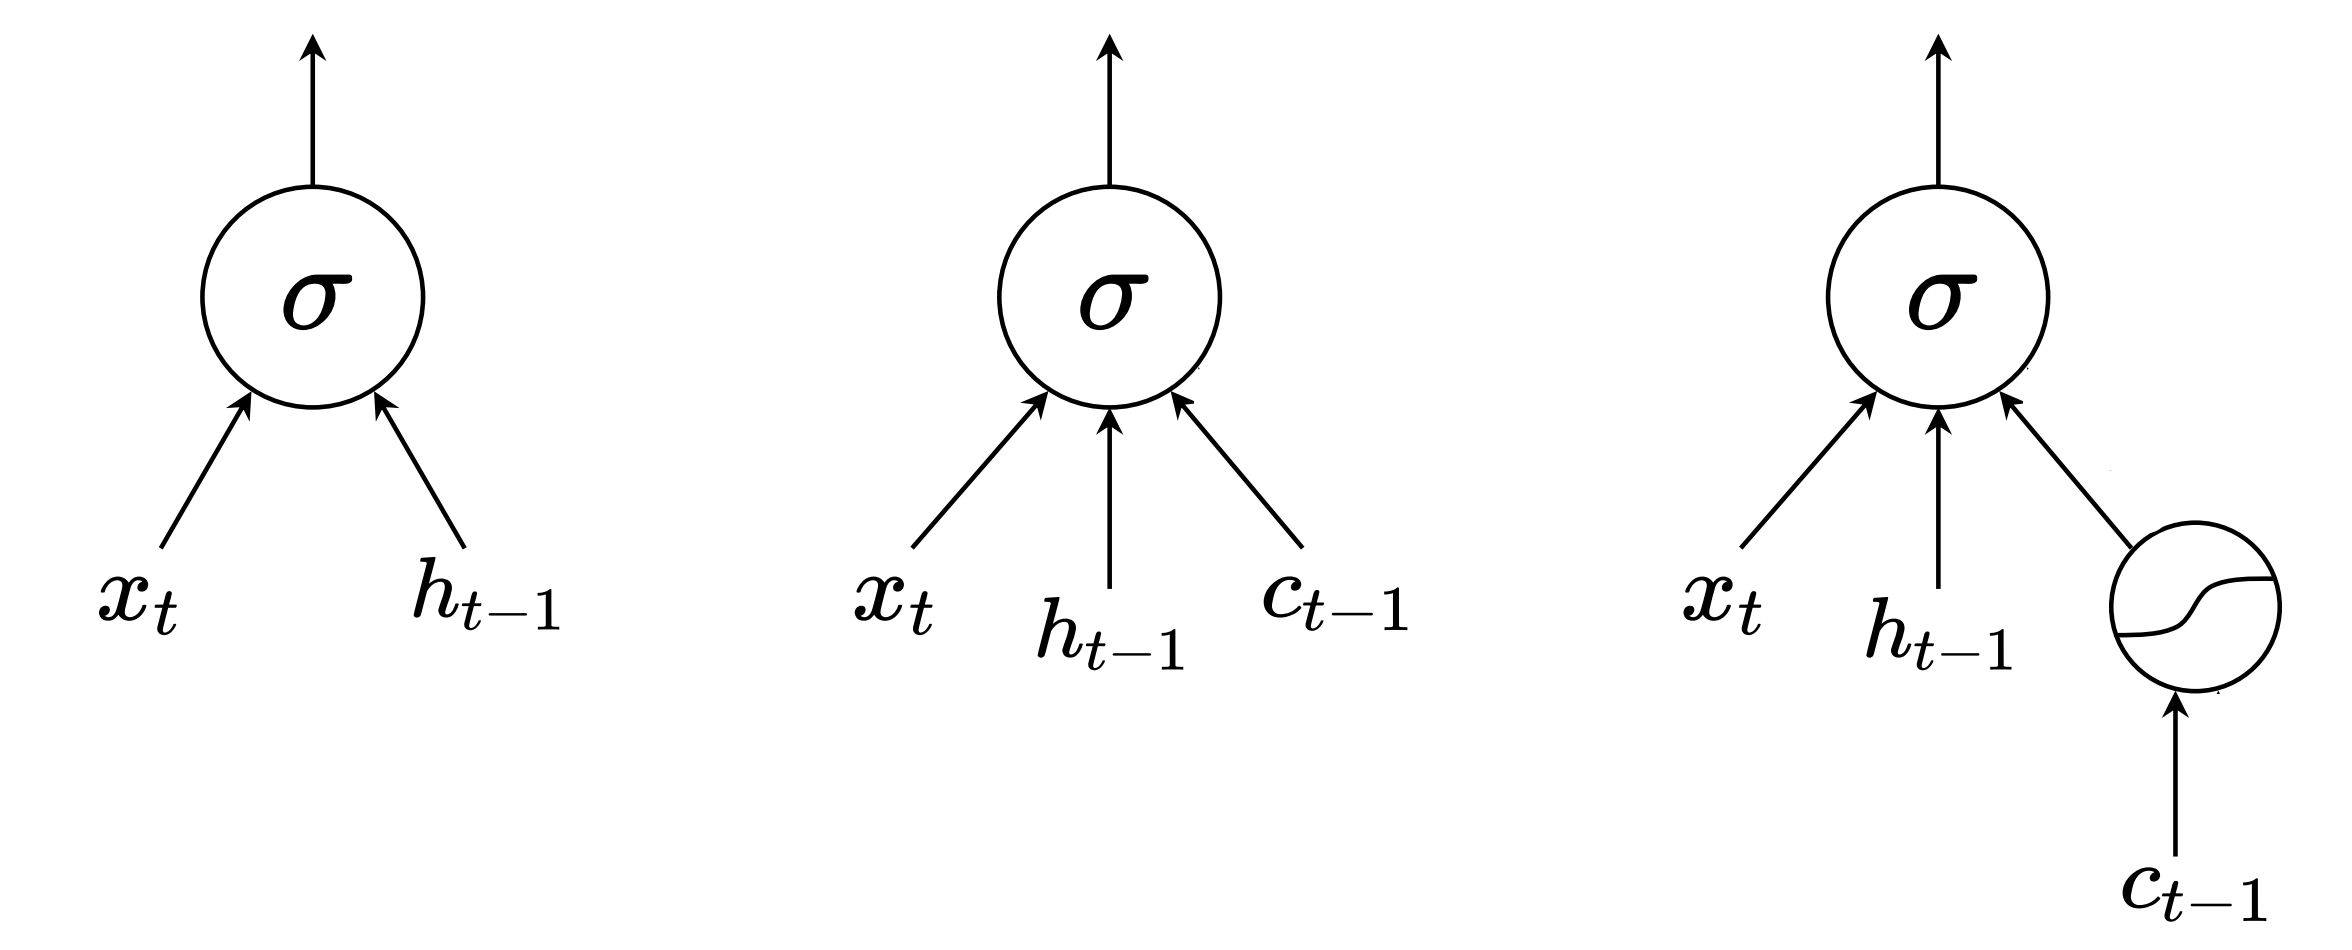
\includegraphics[width=0.8\textwidth]{lstm.png}
    \caption{Comparison between the gate of a vanilla LSTM, peephole LSTM and tanh-LSTM.}
    \label{fig:lstm}
\end{figure}

\begin{enumerate}[(1)]
\item (2 points) Let's first compare the vanilla LSTM and the peephole LSTM. At first glance, adding $\mathbf{c}_{t-1}$ or $\mathbf{c}_t$ to the gate input is redundant, since $\mathbf{h}_t$ is a function of $\mathbf{c}_t$. Explain in what situations would $\mathbf{c}_t$ carry more information than $\mathbf{h}_t$ and is therefore not a redundant term to control the gates.\\
\begin{answertext}{8cm}{}

\end{answertext}

\item \label{q13} (3 points) Let's consider a limitation of the peephole LSTM.
In peephole LSTM, is the range of the value of $\mathbf{x}_t$, $\mathbf{h}_t$ and $\mathbf{c}_t$ bounded or not? How would the value of $\mathbf{c}_t$ change over time, considering its influence on the gates?\\
\begin{answertext}{10cm}{}

\end{answertext}
\newpage
\item \label{q14} (2 points) Give 2 reasons why we don't want a large $\mathbf{c}_t$ during the training of the peephole LSTM. \textit{hint: Consider the gates, and the behavior of the gradient updates on $\mathbf{W}_{*c}$.}\\
\begin{answertext}{10cm}{}

\end{answertext}

\item (2 points) Based on your answers for 1.3 and 1.4, state how tanh-LSTM would improve over peephole LSTM.\\
\begin{answertext}{9cm}{}

\end{answertext}
\end{enumerate}

\newquestion
\section*{\arabic{QuestionCounter}) 
Dataset Shift (7 points)} 
In this question, we will discuss how to compensate for the effect of covariate shift.
\\\\
Consider a training set $\{(\vx_i, \vy_i )\}^n_{i=1}$, where $\vx_i\in\mathcal{X}\subset \mathbb{R}^d$ is an instance drawn i.i.d. from the probability distribution $P_{train}(\vx)$. $\vy_i\in\mathcal{Y}\subset \mathbb{R}$ is the corresponding label following a conditional probability distribution $P(\vy|\vx)$. Let $\ell(\vx, \vy, \hat{\vy}): \mathcal{X} \times \mathcal{Y} \times \mathcal{Y} \xrightarrow[]{} [0, \infty)$ be the loss function, which measures the loss (error) between the true output value $\vy$ for an instance $\vx$ as compared to the estimate $\hat{\vy}$.
\\\\
We will use a parametric model $\hat{f}(\vx)$ for estimating the label $\vy$. Consider a new instance $(\vt, \vec{u})$ that is not in the training set but is part of some future test set. $\vt \in \mathcal{X}$ is a test example and $\vec{u}\in\mathcal{Y}$ is the corresponding label. \\\\
The empirical risk given by leave-one-out cross validation is:
\begin{equation}\label{eq13}
    \hat{R}^{(n)}_L \equiv \frac{1}{n}\sum_{j=1}^n\ell(\vx_j, \vy_j, \hat{f}_j(\vx_j)),
\end{equation}
where $\hat{f}_j$ is a function learned on the training set $\{(\vx_i, \vy_i)\}_{\forall i \in n, i\neq j}$.\\\\
The expected test error over the training instances, which is also known as the \textit{risk} or the generation error, is as follows:
\begin{equation}\label{q14}
    R^{(n-1)} \equiv \mathbb{E}_{\{\vx_i, \vy_i\}_{i\neq j}, \vt, \vec{u}} [\ell(\vt, \vec{u}, \hat{f}_j(\vt))].
\end{equation}
In \textit{standard} supervised learning settings, the test sample $(\vt, \vec{u})$ is assumed to follow $P(\vec{u}|\vt)P_{train}(\vt)$, which is the same probability distribution as for the training samples $\{(\vx_i,\vy_i)\}^n_{i=1}$. In this case, leave-one-out cross validation gives an almost unbiased estimate of the risk, i.e.
\begin{equation}\label{q15}
    \mathbb{E}_{\{\vx_i, \vy_i\}^n_{i=1}}[\hat{R}^{(n)}_L] = R^{(n-1)} \approx R^{(n)}.
\end{equation}
However, Equation (\ref{q15}) does not hold true under the covariate shift, where $\vt$ is not drawn from $P_{train}$.

\begin{enumerate}[(1)]

\item (2 points) Under covariate shift, how do the conditional distribution $P(\vec{u}|\vt)$ and the probability distribution $P_{test}(\vt)$ compare to the \textit{standard} supervised learning setting?\\
\begin{answertext}{6cm}{}

\end{answertext}
\item (5 points) Consider the following weighted empirical risk of leave-one-out cross validation:
\begin{equation}\label{q16}
    \hat{R}^{(n)}_{LW} \equiv  \frac{1}{n}\sum_{j=1}^n \frac{p_{test}(\vx_j)}{p_{train}(\vx_j)}\ell(\vx_j, \vy_j, \hat{f}_j(\vx_j)).
\end{equation}
Show that under the covariate shift,
\begin{equation}\label{q17}
    \mathbb{E}_{\{\vx_i,\vy_i\}^n_{i=1}}[\hat{R}^{(n)}_{LW} ] = R^{(n-1)}.
\end{equation}
\textit{hint: $\mathbb{E}_{\{\vx_i, \vy_i\}^n_{i=1}}[\frac{1}{n}\sum_{j=1}^n g(\vx_j)] = \frac{1}{n}\sum_{j=1}^n \mathbb{E}_{\{\vx_i, \vy_i\}_{i\neq j}, \vx_j, \vy_j} [g(\vx_j)]$, where $g$ can be any function.}\\
\begin{answertext}{19cm}{}

\end{answertext}
\begin{answertext}{23cm}{}
    
\end{answertext}
\end{enumerate}

\newquestion
\section*{\arabic{QuestionCounter}) Evaluation (8 points)}
We are building machine learning models to diagnose a \textbf{rare fatal disease}, where the number of negative samples (healthy people) is much larger than the number of positive samples (sick people).
\begin{enumerate}[(1)]
 \item (4 points) We decide to use $F_{\beta}$ score as the evaluation metric:
    \begin{equation}\label{q19}
        F_{\beta} = (1 + \beta^2) \cdot \frac{\text{precision}\cdot \text{recall}}{(\beta^2\cdot \text{precision}) + \text{recall}},
    \end{equation}
    with $0 < \beta < +\infty$. How would you adjust the value of $\beta$? Explain.\\
    \begin{answertext}{18cm}{}
     
    \end{answertext}
   
    \item (4 points) Suppose we decide to build a logistic regression model with a modified loss function to diagnose the disease:
    \begin{equation}\label{q20}
        L = \frac{1}{n}\sum_{i=1}^n-w_0y_i\log(\hat{y}_i) - w_1(1-y_i)\log(1-\hat{y}_i),
    \end{equation}
    where $y_i$ is the actual probability of a sample $i$ having the disease (a positive sample); $\hat{y}_i$ is model prediction. $w_0 \in [0,1]$, $w_1 \in [0,1]$ are weights for the positive and negative class respectively, and $w_0+w_1=1$. Would you set the value of $w_0$ to be greater, smaller than, or equal to the value of $w_1$? Explain.\\
    \begin{answertext}{18cm}{}
    
    \end{answertext}
\end{enumerate}

\newquestion
\section*{\arabic{QuestionCounter}) Fairness (6 points) } 
We are building a machine learning model to suggest a salary for a person based on the following attributes: gender, age, education, marital-status, occupation, relationship (wife, own-child, husband, unmarried), race, working hours per week, native country. However, the model we obtained is gender biased. Our model's predictions indicate that males on average should have a higher salary than females. In the following questions, we will work on debiasing our model.
\begin{enumerate}[(1)]
    \item (4 points) We first try \textbf{debiasing by unawareness}: we retrain our model on the same dataset but drop the gender attribute, which gives the following confusion matrix:
    \begin{figure}[h]
        \centering
        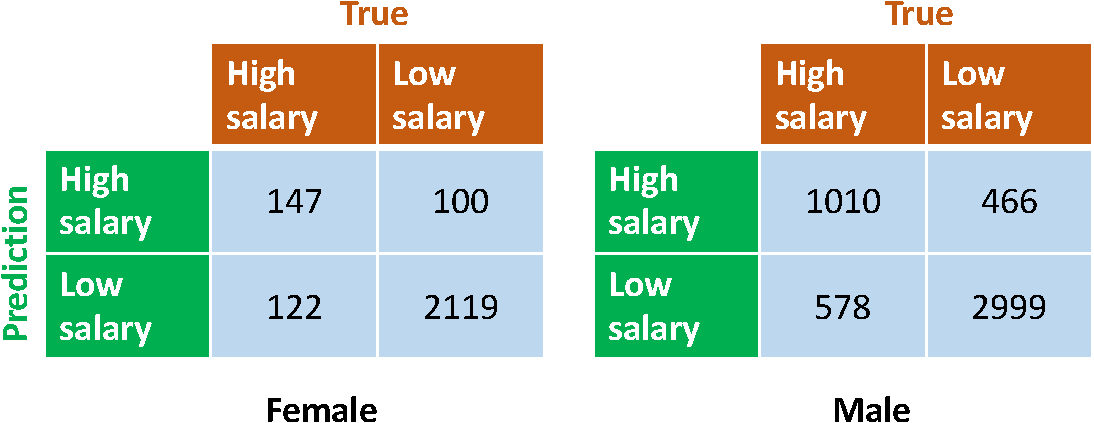
\includegraphics[width=\textwidth]{fairness_unaware.pdf}
    \end{figure} 
    \\Show whether the predictions satisfy \textbf{Statistical/Demographic Parity}. In this question, we assume two numbers A and B are equal if $|A-B|\leq0.05$. Round off your intermediate results to 3 decimal digits.\\
    \begin{answertext}{10cm}{}
   
    \end{answertext}
    
\item (2 points) What are the possible flaws of debiasing by unawareness that limit its ability to improve fairness?\\
\begin{answertext}{20cm}{}

\end{answertext}

\end{enumerate}

\end{document}